\chapter{Теоретическая часть} \label{ch1}

\section{Формат входного сигнала}

В качестве входного сигнала был выбран аудиоформат wav по следующим причинам:
\begin{itemize}
	\item отсутствие сжатия данных;
	\item наличие готовых инструментов для чтения/записи.
\end{itemize}

% не рекомендуется использовать отдельную section <<введение>> после лета 2020 года
%\section{Введение. Сложносоставное название первого параграфа первой главы для~демонстрации переноса слов в содержании} \label{ch1:intro}

\section{Алгоритм генерации сигнала}

DTMF-сигнал представляет собой аддитивную модель двух гармонических процессов \cite{dtmf}:
\begin{equation}
	x_{k}(t) = A_{0} * sin(2*\pi*f_{1}*k*\triangle{t}) + A_{0} * sin(2*\pi*f_{2}*k*\triangle{t}),
\end{equation}

где $k=0,1,...,N-1$, $A_{0}$ - амплитуда сигнала, $f_{1}$ и $f_{2}$ - частоты гармоник, $\triangle{t}$ - шаг дискретизации.

Частоты гармоник берутся по приведённой ниже \taref{tab:lrt} из столбца и строки, соответствующих передаваемому символу. Каждая строка набора представлена частотой низкого тона, а каждый столбец - частотой высокого тона.

\begin{table}[ht]
\centering\small
	\caption{Таблица соответствия частот и символов DTMF \cite{dtmf}}
	\label{tab:lrt}	
\begin{tabular}{|c|c|c|c|l|}
\hline
\multicolumn{1}{|l|}{\textbf{1209 Гц}} & \multicolumn{1}{l|}{\textbf{1336 Гц}} & \multicolumn{1}{l|}{\textbf{1477 Гц}} & \multicolumn{1}{l|}{\textbf{1633 Гц}} &                 \\ \hline
1                                      & 2                                     & 3                                     & A                                     & \textbf{697 Гц} \\ \hline
4                                      & 5                                     & 6                                     & B                                     & \textbf{770 Гц} \\ \hline
7                                      & 8                                     & 9                                     & C                                     & \textbf{852 Гц} \\ \hline
*                                      & 0                                     & \#                                    & D                                     & \textbf{941 Гц} \\ \hline
\end{tabular}\normalsize% возвращаем шрифт к нормальному
\end{table}

Шаг дискретизации определяется, как отношение единицы к частоте дискретизации (rate) \cite{bel}. Согласно стандарту, для DTMF-сигнала приемлемым значением rate является 8000 Гц \cite{dtmf}. Однако это не необходимость: можно выбрать и более высокую частоту дискретизации - в конечном итоге это влияет больше на время вычислений (кодирования \/ декодирования сигнала). Чтобы уменьшить время подсчета частот далее воспользуемся рекомендациями стандарта и будем использовать частоту дискретизации - 8000 Гц.

Сам процесс генерации сообщения двухтонального многочастотного набора заключается в последовательной генерации множества значений гармоник для каждого символа сообщения с последующей записью в файл.

\section{Декодирование сигнала DTMF}

Опишем базовый алгоритм декодирования сигнала. Представим, что мы записали в wav-файл звук символов $"3*33"$, как показано на \firef{fig:step-1}.

\begin{figure}[ht] 
	\center
	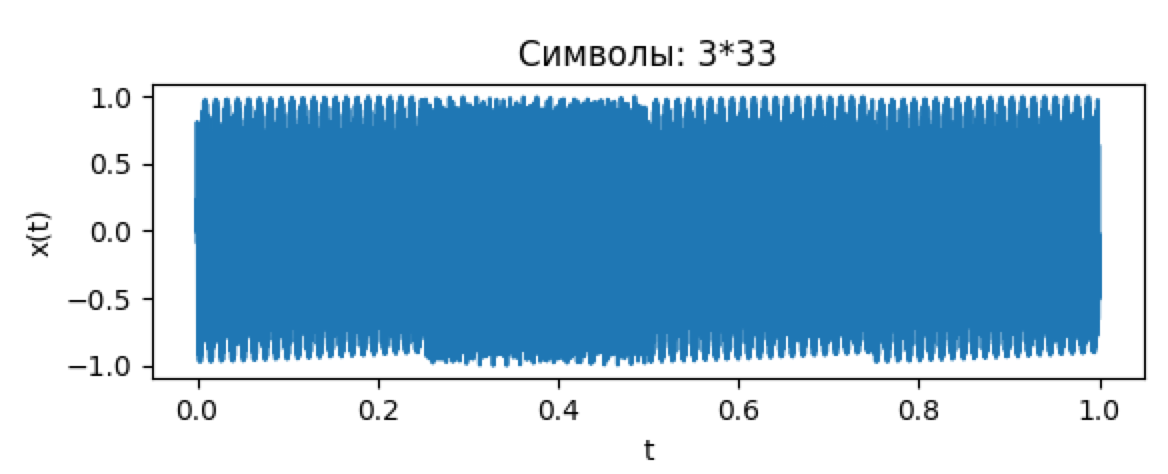
\includegraphics [scale=0.7] {my_folder/images/step-1}
	\caption{График сигнала $"3*33"$} 
	\label{fig:step-1}
	\end{figure}

С помощью спектра Фурье на \firef{fig:step-2} мы можем увидеть набор частот, используемых в нашем сообщении, и даже то, как часто они повторяются исходя из амплитуды определенных частот: 

\begin{figure}[ht] 
	\center
	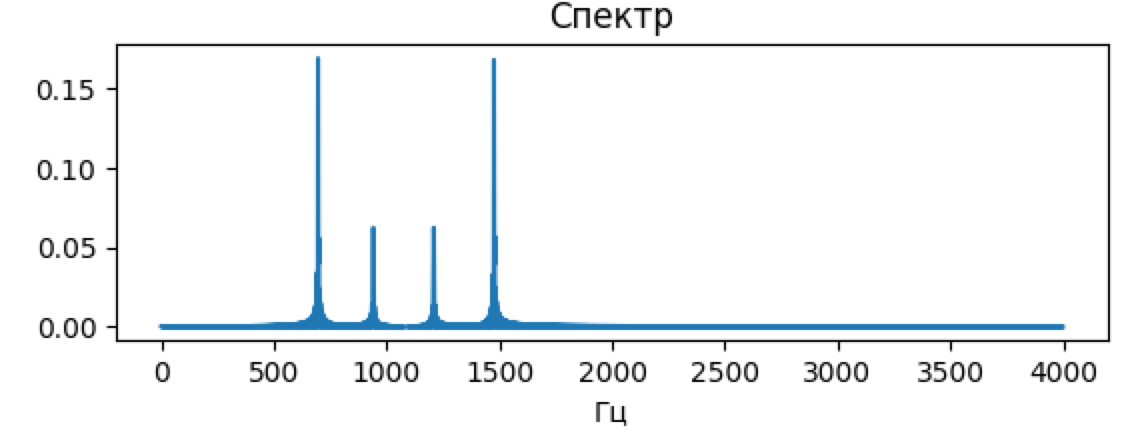
\includegraphics [scale=0.7] {my_folder/images/step-2}
	\caption{Спектр сигнала $"3*33"$} 
	\label{fig:step-2}
	\end{figure}
	
Минусом подобного решения в лоб является то, что мы не можем определить порядок символов в сообщении. Чтобы это исправить, можно обрабатывать сигнал пачками - мы заранее знаем, сколько секунд длится каждый сигнал, поэтому нам не составит труда для каждого отрезка построить спектр и извлечь из него необходимые частоты.

На примере выше, каждый сигнал длится по 0,25 секунд, поэтому размер одной такой пачки обработки будет равен произведению времени одного сигнала на частоту дискретизации. Вот полученные значения второго символа на \firef{fig:step-4}:

\begin{figure}[ht] 
	\center
	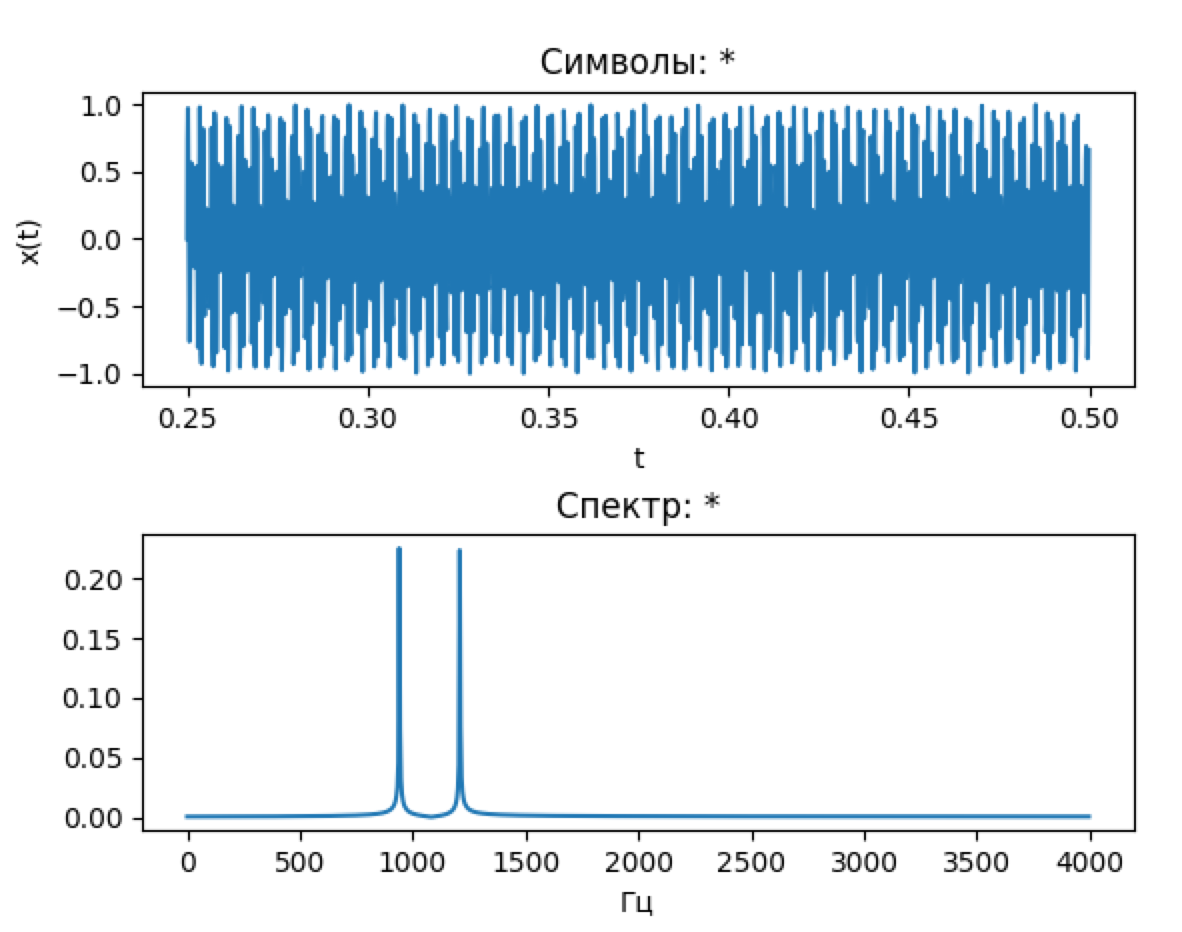
\includegraphics [scale=0.6] {my_folder/images/step-4}
	\caption{Спектр сигнала $"*"$} 
	\label{fig:step-4}
	\end{figure}

Недостатком примитивного решения является - скорость. К сожалению, подсчет спектра для каждой пачки значений достаточно дорогостоящая по времени операция, особенно при увеличении частоты дискретизации. Поэтому воспользуемся специальными алгоритмами преобразования Фурье.

Для решения задачи детектирования и декодирования тональных сигналов в телефонии обычно применяются две вариации дискретного преобразования Фурье: быстрое преобразование Фурье (FFT) и алгоритм Гёрцеля. 

В рамках данной работы воспользуемся последней, так как в отличие от быстрого преобразования Фурье, вычисляющего все частотные компоненты ДПФ, нам уже заранее известны частотные компоненты, которые мы хотим найти.

Алгоритм Гёрцеля заключается в следующем. Пусть $x_{n},\ n=0,\dots ,N-1$ — измеренные значения сигнала, которые являются входными данными для дискретного преобразования Фурье, а $X_{k},\ k=0,\dots ,N-1$ — частотные компоненты дискретного преобразования Фурье, так как нам не важны их фазы будем искать магнитуды $X_{k}^{2}$.

Для расчёта $X_{k}^{2}$ с помощью алгоритма Гёрцеля последовательно вычисляются члены последовательности $s_n$ для $n=0, ..., N-1$ по рекуррентной формуле:
\begin{equation}
 	s_{n}=2\cos \left({\frac {2\pi k}{N}}\right)s_{n-1}-s_{n-2}+x_{n}, \cite{dtmf}
\end{equation}	
где $s_{-1}=s_{-2}=0$, $k_n = [0.5 + \frac{n * N}{rate}]$.

Искомое значение получается как:
\begin{equation}
	X_{k}^{2}=s_{N-1}^{2}-2\cos \left({\frac {2\pi k}{N}}\right)s_{N-1}s_{N-2}+s_{N-2}^{2}.
\end{equation}	

Найденные частоты сопоставляются с частотной \taref{tab:lrt}.

Алгоритм Гёрцеля позволяет эффективно работать с достаточно высокими частотами дискретизации, например, 22050 или 44100.

\section{Выводы} \label{ch1:conclusion}

В рамках данной главы был выбран аудио-формат wav для работы со сгенерированными звуковыми сигналами.

Рассмотрели способ кодирования сообщений в соответсвии с приведенной \taref{tab:lrt}, а также подобрали частоту дискретизации для эффективного, с пррактической точки зрения, кодирования сообщения.

Для декодирования исследовали три варианта поиска частотных компонент: дискретное преобразование Фурье, быстрое преобразование Фурье и алгоритм Гёрцеля. Как итог, выбрали последний, так как он требует меньшего количества операций для расчета частотных компонент.

Рассмотрим практическую реализацию алгоритмов кодирования и декодирования DTMF-сигналов в следующей главе. 

%% Вспомогательные команды - Additional commands
%
\newpage % принудительное начало с новой страницы, использовать только в конце раздела
%\clearpage % осуществляется пакетом <<placeins>> в пределах секций
%\newpage\leavevmode\thispagestyle{empty}\newpage % 100 % начало новой страницы